\chapter{Temperature-dependent ATDHFB}

A lot of these ideas I'm getting from \cite{Schunck2015FTfission} as well as Nicolas' own temperature-dependent HFB notes.

\section{A brief overview of the theory}

As in any statistical theory, one first must determine which sort of ensemble properly describes the system. Nuclei have (in principle) conserved number of particles; however in HFB theory, that's somewhat flexible since the BCS transformation explicitly breaks particle number symmetry. In principle we should perhaps use a microcanonical ensemble to describe a nucleus as a closed, isolated system, but that turns out to be challenging to solve because it requires a full knowledge of the eigenspectrum of the nucleus. Using that quirk of HFB theory, we wiggle our way out of this hairiness\footnote{You can wave your hands here and say that finite temperatures let you break superfluid pairs, and so the number of ``quasiparticles" (which you could argue might have referred to pairs before but now might also include individual particles) can change.} to instead describe our system using the grand canonical ensemble, and this turns out to be tractable.

Moving forward by minimizing the grand potential $\Omega$ gives us for the density:
\begin{equation*}
\hat{D} = \frac{1}{Z}e^{-\beta\left(\hat{H}-\mu\hat{N}\right)}
\end{equation*}

\noindent with associated partition function

\begin{equation*}
Z = Tr\left[e^{-\beta\left(\hat{H}-\mu\hat{N}\right)}\right]
\end{equation*}

Getting specifically to our particular choice of mean-field Hamiltonian, we substitute in some one-body operator for the exponent:

\begin{equation*}
\hat{D}_{HF} = \frac{1}{Z}e^{-\beta\hat{K}}, Z = Tr\left[e^{-\beta\hat{K}}\right]
\end{equation*}

\noindent where in the plain ol' Hartree Fock case, $\hat{K} = \sum_{ij}K_{ij}c_i^\dagger c_j$ (in the HFB case, $\hat{K}$ is a sum of all different one-body operator types, but it's the same basic idea).

Defining the HF density matrix $\rho_{ij}=Tr\left[\hat{D}_{HF}c_j^\dagger c_i\right]$, we can show the following useful correspondence relations:

\begin{align*}
\rho &= \frac{1}{1+e^{\beta\hat{K}}} \\
Tr\left[\hat{D}_{HF}\hat{A}\right] &= tr\left[\rho\hat{A}\right] = \sum_{ij}\rho_{ij}\hat{A}_{ij}
\end{align*}

\noindent where $\hat{A}$ is some operator in the single-particle basis. Similar things happen for the HFB case. At the end of the day in HFB, things work out to be pretty similar to the way they were before, except the density in the quasiparticle basis is replaced by

\begin{equation*}
\mathcal{R} =
\left(\begin{array}{cc}
0 & 0 \\
0 & 1
\end{array}\right)
\rightarrow
\left(\begin{array}{cc}
f & 0 \\
0 & 1-f
\end{array}\right)
\end{equation*}

\noindent with the Fermi factor $f$ given by $f_\mu=\frac{1}{1+e^{\beta E_\mu}}$. Obviously there's a lot more richness to it than that, but this helps to at least see the basic skeleton of what changes at finite temperature.

\section{Temperature-Dependent ATDHFB}

Let us quickly review the essence of Time-Dependent Hartree-Fock-Bogoliubov (TDHFB). The fundamental assumption of TDHFB is that a system which is a Slater determinant at time $t=0$ and which is then allowed to evolve in time will remain a Slater determinant at all times $t$. This assumption allows us to write to TDHFB equation:

\begin{equation*}
i\hbar \mathcal{\dot{R}} = \left[\mathcal{H},\mathcal{R}\right]
\end{equation*}

\noindent where in the single-particle basis

\begin{equation*}
\mathcal{\tilde{H}} = 
\left(\begin{array}{cc}
h-\lambda & \Delta \\
-\Delta^* & -h^*+\lambda
\end{array}\right), 
\qquad \mathcal{\tilde{R}} = 
\left(\begin{array}{cc}
\rho & \kappa \\
-\kappa^* & 1-\rho^*
\end{array}\right)
\end{equation*}

The \textit{additional} assumption that collective motion is slow compared to single particle motion of the system is called the \textit{adiabtic approximation}, and the consequent model is called Adiabatic Time-Dependent Hartree-Fock-Bogoliubov (ATDHFB). Historically, the reason for this assumption comes from microscopic-macroscopic models of nuclear fission, where the dynamics of the system are described by a few collective shape variables and their derivatives (you might think of them semiclassically as coordinates and velocities). The adiabatic approximation is implicit in this assumption. ATDHFB provides the bridge for bringing this useful framework into a self-consistent, fully-microscopic picture.

Once the system is described in terms of collective coordinates and velocities, the energy can be expressed as the sum of a ``potential" term (which depends on the coordinates) and a ``kinetic" term (which depends on the velocities). Our goal is to understand the kinetic part of the energy, which in some sense describes the dynamics of, for example, a fissioning nucleus, in terms of the first few multipole moments of the nucleus. A key component of this will be the inertia tensor $\mathcal{M}$, which plays the role of the ``mass": $E_{kin}\sim\frac{1}{2}\mathcal{M}\dot{q}^2$

\subsection{Review of ATDHFB}

With the adiabatic assumption in place, we can write the density as an expansion around some time-even zeroth-order density:

\begin{align*}
\mathcal{R}(t) 
&= e^{i\chi(t)}\mathcal{R}_0(t)e^{-i\chi(t)} \\
&= \mathcal{R}_0 + \mathcal{R}_1 + \mathcal{R}_2 + \dots
\end{align*}

\noindent where $\chi$ is assumed to be ``small" (which is explained more rigorously in \cite{Baranger1978}) and

\begin{align}\label{eqn:densities}
\mathcal{R}_1 &= i\left[\chi, \mathcal{R}_0\right] \\
\mathcal{R}_2 &= \frac{1}{2}\left[\left[\chi, \mathcal{R}_0\right], \chi\right] 
\end{align}

\noindent The HFB matrix, being a function of $\mathcal{R}$, is likewise expanded:

\begin{equation*}
\mathcal{H} = \mathcal{H}_0 + \mathcal{H}_1 + \mathcal{H}_2 + \dots
\end{equation*}

\noindent and together $\mathcal{R}$ and $\mathcal{H}$ are plugged into the TDHFB equation. Gathering terms in powers of $\chi$:

\begin{align}\label{eqn:ATDHFB_eqns}
i\hbar\mathcal{\dot{R}}_0 &= \left[\mathcal{H}_0, \mathcal{R}_1\right] + \left[\mathcal{H}_1, \mathcal{R}_0\right] \\
i\hbar\mathcal{\dot{R}}_1 &= \left[\mathcal{H}_0, \mathcal{R}_0\right] + \left[\mathcal{H}_0, \mathcal{R}_2\right]
 + \left[\mathcal{H}_1, \mathcal{R}_1\right] + \left[\mathcal{H}_2, \mathcal{R}_0\right]
\end{align}

\noindent These two equations are the ATDHFB equations. They can be solved self-consistently to find both $\chi$ and $\mathcal{R}_0$; however, this is rarely done in practice. More commonly what is done is to exploit the fact that solutions to the ATDHFB equations are (by design) \textit{close} to true HFB solutions. We then take HFB solutions and compute their time derivatives by the first ATDHFB equation to get ATDHFB-like behavior without going through the full trouble of ATDHFB.

One nice feature of using true HFB solutions instead of ATDHFB solutions is that the matrix $\mathcal{H}_0$ is diagonal in the HFB basis.

Finally, the total energy of the system is found to be

\begin{equation*}
E(\mathcal{R}) = E_{HFB} + \frac{1}{2}\mathrm{Tr}\left(\mathcal{H}_0\mathcal{R}_1\right) + \frac{1}{2}\mathrm{Tr}\left(\mathcal{H}_0\mathcal{R}_2\right) + \frac{1}{4}\mathrm{Tr}\left(\mathcal{H}_1\mathcal{R}_1\right)
\end{equation*}

\noindent The ``kinetic energy" of the system is given by the latter two terms, which (as I'll show explicitly in a moment), are both second order in $\chi$.

\subsection{Relation between $\chi$ and $\dot{\mathcal{R}}$}\label{sect:chi-rdot}

Eventually we'll want to express the energy in terms of the multipole moments $q$ and their derivatives, but for now we will content ourselves with expressing the energy in terms of $\mathcal{R}$ and $\dot{\mathcal{R}}$. From the first ATDHFB equation:

\begin{equation*}
i\hbar\mathcal{\dot{R}}_0 = \left[\mathcal{H}_0, \mathcal{R}_1\right] + \left[\mathcal{H}_1, \mathcal{R}_0\right]
\end{equation*}

Working in the HFB quasiparticle basis, we have (at finite temperatures)

\begin{equation*}
\mathcal{H}_0 = 
\left(\begin{array}{cc}
E & 0 \\
0 & -E
\end{array}\right), 
\qquad \mathcal{R}_0 = 
\left(\begin{array}{cc}
f & 0 \\
0 & 1-f
\end{array}\right)
\end{equation*}

\noindent Note that the block matrices $E$ and $f$ are both diagonal. In this same basis, we can also divide the perturbation matrix $\chi$ and the first-order energy $\mathcal{H}_1$ in the same block matrix form:

\begin{equation*}
\qquad \chi = 
\left(\begin{array}{cc}
\chi^{11} & \chi^{12} \\
\chi^{21} & \chi^{22}
\end{array}\right),
\qquad \mathcal{H}_1 = 
\left(\begin{array}{cc}
\mathcal{H}_1^{11} & \mathcal{H}_1^{12} \\
\mathcal{H}_1^{21} & \mathcal{H}_1^{22}
\end{array}\right)
\end{equation*}

\noindent Ultimately, by using the equations \ref{eqn:densities}, we arrive at the result:

\begin{align}\label{eqn:chi-rdot_uncranked}
\begin{aligned}
\hbar \dot{\mathcal{R}}_{(0),ab}^{11} &= (E_a-E_b)(f_b-f_a)\chi_{ab}^{11} + (f_b-f_a)\mathcal{H}^{11}_{(1),ab} \\
\hbar \dot{\mathcal{R}}_{(0),ab}^{12} &= (E_a+E_b)\left(1-(f_a+f_b)\right)\chi_{ab}^{12} + \left(1-(f_a+f_b)\right)\mathcal{H}^{12}_{(1),ab} \\
\hbar \dot{\mathcal{R}}_{(0),ab}^{21} &= (E_a+E_b)\left(1-(f_a+f_b)\right)\chi_{ab}^{21} - \left(1-(f_a+f_b)\right)\mathcal{H}^{21}_{(1),ab} \\
\hbar \dot{\mathcal{R}}_{(0),ab}^{22} &= (E_a-E_b)(f_b-f_a)\chi_{ab}^{22} - (f_b-f_a)\mathcal{H}^{22}_{(1),ab}
\end{aligned}
\end{align}

It is common (the so-called ``cranking approximation") to assume that changes in the density have approximately no effect on the mean field, in which case these relations reduce to

\begin{tcolorbox}
\begin{align}\label{eqn:chi-rdot}
\begin{aligned}
\hbar \dot{\mathcal{R}}_{(0),ab}^{11} &= (E_a-E_b)(f_b-f_a)\chi_{ab}^{11} \\
\hbar \dot{\mathcal{R}}_{(0),ab}^{12} &= (E_a+E_b)\left(1-(f_a+f_b)\right)\chi_{ab}^{12} \\
\hbar \dot{\mathcal{R}}_{(0),ab}^{21} &= (E_a+E_b)\left(1-(f_a+f_b)\right)\chi_{ab}^{21} \\
\hbar \dot{\mathcal{R}}_{(0),ab}^{22} &= (E_a-E_b)(f_b-f_a)\chi_{ab}^{22}
\end{aligned}
\end{align}
\end{tcolorbox}

\noindent\textit{Sanity Check:} In the $T=f=0$ case, the $^{11}$ and $^{22}$ terms vanish completely and we are left with the familiar [zero-temperature] ATDHFB equations:

\begin{align*}
\hbar \dot{\mathcal{R}}_{(0),ab}^{12} &= (E_a+E_b)\chi_{ab}^{12} + \mathcal{H}^{12}_{(1),ab} \\
\hbar \dot{\mathcal{R}}_{(0),ab}^{21} &= (E_a+E_b)\chi_{ab}^{21} - \mathcal{H}^{21}_{(1),ab}
\end{align*}

Another thing we must be careful of is the case of degenerate states. In such an event, $E_a=E_b$ and $f_a=f_b$, leading again to $\mathcal{\dot{R}}^{11}_{(0),ab}=\mathcal{\dot{R}}^{22}_{(0),ab}=0$ (but I emphasize that this is only for this particular pair of states $|a\rangle$ and $|b\rangle$).

A third, rather pedantic case to be aware of is the example of a two-state system. In that case, $f_a+f_b=1$ and then the opposite happens; namely, $\mathcal{\dot{R}}^{12}_{(0),ab}=\mathcal{\dot{R}}^{21}_{(0),ab}=0$ while $\mathcal{\dot{R}}^{11}_{(0),ab}\neq0, \mathcal{\dot{R}}^{22}_{(0),ab}\neq0$

\subsection{Kinetic Energy at Finite Temperature}

As mentioned previously, the expression for the ``kinetic" energy of the system is given by:

\begin{equation*}
E_{kin}(\mathcal{R}) = \frac{1}{2}\mathrm{Tr}\left(\mathcal{H}_0\mathcal{R}_2\right) + \frac{1}{4}\mathrm{Tr}\left(\mathcal{H}_1\mathcal{R}_1\right)
\end{equation*}

\subsubsection{Term proportional to $\mathcal{R}_2$}

It can be shown that

\begin{equation*}
\mathrm{Tr}\left(\mathcal{H}_0\mathcal{R}_2\right) = \frac{1}{2}\mathrm{Tr}\left(\left[\chi,\mathcal{H}_0\right]\left[\chi,\mathcal{R}_0\right]\right)
\end{equation*}

\noindent which leads to

\begin{equation*}
\left[\chi, \mathcal{H}_0\right] = \left(\begin{array}{cc}
[\chi^{11},E] & -\left\{\chi^{12},E\right\} \\
\left\{\chi^{21},E\right\} & -[\chi^{22},E]
\end{array}\right), \qquad
\left[\chi, \mathcal{R}_0\right] = \left(\begin{array}{cc}
[\chi^{11},f] & \chi^{12}-\left\{\chi^{12},f\right\} \\
-\chi^{21}+\left\{\chi^{21},f\right\} & -[\chi^{22},f]
\end{array}\right)
\end{equation*}

\begin{align}\label{eqn:H0R2}
\begin{aligned}
\mathrm{Tr}\left(\mathcal{H}_0\mathcal{R}_2\right) = \frac{1}{2}
&\mathrm{Tr} \left([\chi^{11},E][\chi^{11},f] + \left\{\chi^{12},E\right\}(\chi^{21}-\{\chi^{21},f\})\right. \\
&\left.+ \left\{\chi^{21},E\right\}(\chi^{12}-\{\chi^{12},f\}) + [\chi^{22},E][\chi^{22},f]\right)
\end{aligned}
\end{align}

Since $E$ and $f$ are diagonal, we can simplify expressions involving commutators and anticommutators. If $A$ is an arbitrary matrix and $D$ is diagonal, then

\begin{align*}
[A,D]_{\mu\nu} &= (D_\nu-D_\mu)A_{\mu\nu} \\
\left\{A,D\right\}_{\mu\nu} &= (D_\mu+D_\nu)A_{\mu\nu} \\
A_{\mu\nu}-\left\{A,D\right\}_{\mu\nu} &= (1-D_\mu-D_\nu)A_{\mu\nu}
\end{align*}

\noindent Then this energy term becomes

\begin{align*}
\frac{1}{2}\mathrm{Tr}\left(\mathcal{H}_0\mathcal{R}_2\right) = \frac{1}{4}
& \left[(E_b-E_a)(f_a-f_b)\chi^{11}_{ab}\chi^{11}_{ba} + (E_a+E_b)(1-f_a-f_b)\chi^{12}_{ab}\chi^{21}_{ba}\right. \\
&\left.+ (E_a+E_b)(1-f_a-f_b)\chi^{21}_{ab}\chi^{12}_{ba} + (E_b-E_a)(f_a-f_b)\chi^{22}_{ab}\chi^{22}_{ba}\right]
\end{align*}

\noindent If you wanted to get \textit{really} crazy (and we'll see in a bit why this might actually be okay), you could even throw in some extra delta functions to get this:

\begin{align*}
\frac{1}{2}\mathrm{Tr}\left(\mathcal{H}_0\mathcal{R}_2\right) = \frac{1}{4}
& \left[(E_b-E_a)(f_a-f_b)\delta_{a\alpha}\delta_{b\beta}\chi^{11}_{\alpha\beta}\chi^{11}_{ba} + (E_a+E_b)(1-f_a-f_b)\delta_{a\alpha}\delta_{b\beta}\chi^{12}_{\alpha\beta}\chi^{21}_{ba}\right. \\
&\left.+ (E_a+E_b)(1-f_a-f_b)\delta_{a\alpha}\delta_{b\beta}\chi^{21}_{\alpha\beta}\chi^{12}_{ba} + (E_b-E_a)(f_a-f_b)\delta_{a\alpha}\delta_{b\beta}\chi^{22}_{\alpha\beta}\chi^{22}_{ba}\right]
\end{align*}

\noindent Note that this now has the general form

\begin{tcolorbox}
\begin{align}\label{eqn:H0R2_inertia}
\frac{1}{2}\mathrm{Tr}\left(\mathcal{H}_0\mathcal{R}_2\right) = &
 \mathcal{\bar{M'}}^{11,11}_{\alpha\beta ab}\chi^{11}_{\alpha\beta}\chi^{11}_{ba} +
 \mathcal{\bar{M'}}^{12,21}_{\alpha\beta ab}\chi^{12}_{\alpha\beta}\chi^{21}_{ba} +
 \mathcal{\bar{M'}}^{21,12}_{\alpha\beta ab}\chi^{21}_{\alpha\beta}\chi^{12}_{ba} +
 \mathcal{\bar{M'}}^{22,22}_{\alpha\beta ab}\chi^{22}_{\alpha\beta}\chi^{22}_{ba}
\end{align}
\end{tcolorbox}

\noindent where everything that isn't a $\chi$ has just been kind of absorbed into a single coefficient.

Let's pause here for just a second and think about what we just did. Remember that our goal all along has been to treat this piece of the energy as sort of a ``kinetic energy term" describing motion in a space of collective shape deformation coordinates. Then just now we found that, sure enough, we can factor this particular chunk into something that looks \textit{kind of} like $\frac{1}{2}mv^2$. And we already know from \ref{eqn:chi-rdot} that $\chi$ is related to $\mathcal{\dot{R}}_0$. Eventually we'll try to relate $\mathcal{\dot{R}}_0$ to the collective shape coordinates $\dot{q}$, but first let's see if we can't get the other piece of the kinetic energy into the same form.

\subsubsection{Term proportional to $\mathcal{R}_1$}

Recall that $\mathcal{R}_1 = i\left[\chi, \mathcal{R}_0\right]$; then we can almost copy from equation \ref{eqn:H0R2} of the previous section:

\begin{align}\label{eqn:H1R1}
\frac{1}{4}\mathrm{Tr}\left(\mathcal{H}_{1}\mathcal{R}_{1}\right) = \frac{i}{4}
&\mathrm{Tr} \left(\mathcal{H}_{1}^{11}[\chi^{11},f] - \mathcal{H}_{1}^{12}(\chi^{21}-\{\chi^{21},f\}) \right. \nonumber\\
&\left.+ \mathcal{H}_{1}^{21}(\chi^{12}-\{\chi^{12},f\}) - \mathcal{H}_{1}^{22}[\chi^{22},f]\right) \nonumber\\
= \frac{i}{4}
& \left(\mathcal{H}_{(1),ab}^{11}(f_a-f_b)\chi^{11}_{ba} - \mathcal{H}_{(1),ab}^{12}(1-f_a-f_b)\chi^{21}_{ba} \right. \nonumber\\
&\left.+ \mathcal{H}_{(1),ab}^{21}(1-f_a-f_b)\chi^{12}_{ba} - \mathcal{H}_{(1),ab}^{22}(f_a-f_b)\chi^{22}_{ba}\right)
\end{align}

\noindent But what are those $\mathcal{H}^{1}$ terms? Since the interaction is known in the single-particle basis, we'll have to transform our density into the single-particle basis $\mathcal{R}_1\rightarrow\mathcal{\tilde{R}}_1$, evaluate $\mathcal{\tilde{H}}_1$ (which depends on $\mathcal{\tilde{R}}_1$) in this basis, and then transform the result back into the quasiparticle basis $\mathcal{\tilde{H}}_1\rightarrow\mathcal{H}_1$

\begin{equation*}
\mathcal{\tilde{R}}_1 = \left(\begin{array}{cc}
\rho_1 & \kappa_1 \\
-\kappa_1^* & -\rho_1^*
\end{array}\right) = 
i\left(\begin{array}{cc}
U & V^* \\
V & U^*
\end{array}\right)
\left(\begin{array}{cc}
[\chi^{11},f] & \chi^{12}-\left\{\chi^{12},f\right\} \\
-\chi^{21}+\left\{\chi^{21},f\right\} & -[\chi^{22},f]
\end{array}\right)
\left(\begin{array}{cc}
U^\dagger & V^\dagger \\
V^T & U^T
\end{array}\right)
\end{equation*}

\begin{align*}
\Rightarrow \quad
& \rho_1 = i\left(U[\chi^{11},f]U^\dagger + U\left(\chi^{12}-\left\{\chi^{12},f\right\}\right)V^T - V^*\left(\chi^{21}-\left\{\chi^{21},f\right\}\right)U^\dagger - V^*[\chi^{22},f]V^T \right) \\
& \kappa_1 = i\left(U[\chi^{11},f]V^\dagger + U\left(\chi^{12}-\left\{\chi^{12},f\right\}\right)U^T - V^*\left(\chi^{21}-\left\{\chi^{21},f\right\}\right)V^\dagger - V^*[\chi^{22},f]U^T \right)
\end{align*}

In the single-particle basis, we can compute the interaction mean field $\Gamma_{(1),ij} = \bar{V}_{ikjl}\rho_{(1),lk}$ and the pairing field $\Delta_{(1),ij} = \frac{1}{2}\bar{V}_{ijkl}\kappa_{(1),kl}$:

\begin{align*}
\Gamma_{(1),ij} 
&= \bar{v}_{ikjl}\rho_{(1),lk} \\
&= i\bar{v}_{ikjl}\left(U_{l\alpha}[\chi^{11},f]_{\alpha\beta}U^\dagger_{\beta k} + U_{l\alpha}\left(\chi^{12}-\left\{\chi^{12},f\right\}\right)_{\alpha\beta}V^T_{\beta k}\right. \\
&\left.\qquad - V^*_{l\alpha}\left(\chi^{21}-\left\{\chi^{21},f\right\}\right)_{\alpha\beta}U^\dagger_{\beta k} - V^*_{l\alpha}[\chi^{22},f]_{\alpha\beta}V^T_{\beta k} \right) \\
\Delta_{(1),ij} 
&= \frac{1}{2}\bar{v}_{ijkl}\kappa_{(1),kl} \\
&= \frac{i}{2}\bar{v}_{ijkl}\left(U_{l\alpha}[\chi^{11},f]_{\alpha\beta}V^\dagger_{\beta k} + U_{l\alpha}\left(\chi^{12}-\left\{\chi^{12},f\right\}\right)_{\alpha\beta}U^T_{\beta k}\right. \\
&\left.\qquad - V^*_{l\alpha}\left(\chi^{21}-\left\{\chi^{21},f\right\}\right)_{\alpha\beta}V^\dagger_{\beta k} - V^*_{l\alpha}[\chi^{22},f]_{\alpha\beta}U^T_{\beta k} \right)
\end{align*}

To clean up the presentation a bit, let us introduce the following:

\begin{tcolorbox}
\begin{align*}
J^{11}_{ij\alpha\beta} = i\bar{v}_{ikjl}U_{l\alpha}U^\dagger_{\beta k} &\qquad J^{22}_{ij\alpha\beta} = -i\bar{v}_{ikjl}V^*_{l\alpha}V^T_{\beta k} \\
K^{12}_{ij\alpha\beta} = i\bar{v}_{ikjl}U_{l\alpha}V^T_{\beta k} &\qquad K^{21}_{ij\alpha\beta} = -i\bar{v}_{ikjl}V^*_{l\alpha}U^\dagger_{\beta k} \\
L^{12}_{ij\alpha\beta} = i\bar{v}_{ijkl}U_{l\alpha}U^T_{\beta k} &\qquad L^{21}_{ij\alpha\beta} = -i\bar{v}_{ijkl}V^*_{l\alpha}V^\dagger_{\beta k} \\
M^{11}_{ij\alpha\beta} = i\bar{v}_{ijkl}U_{l\alpha}V^\dagger_{\beta k} &\qquad M^{22}_{ij\alpha\beta} = -i\bar{v}_{ijkl}V^*_{l\alpha}U^T_{\beta k}
\end{align*}
\end{tcolorbox}

\noindent Then the fields simplify to

\begin{align*}
\Gamma_{(1),ij} &= J^{11}_{ij\alpha\beta}[\chi^{11},f]_{\alpha\beta} + K^{12}_{ij\alpha\beta}\left(\chi^{12}-\left\{\chi^{12},f\right\}\right)_{\alpha\beta} + K^{12}_{ij\alpha\beta}\left(\chi^{21}-\left\{\chi^{21},f\right\}\right)_{\alpha\beta} + J^{22}_{ij\alpha\beta}[\chi^{22},f]_{\alpha\beta} \\
2\Delta_{(1),ij}  &= M^{11}_{ij\alpha\beta}[\chi^{11},f]_{\alpha\beta} + L^{12}_{ij\alpha\beta}\left(\chi^{12}-\left\{\chi^{12},f\right\}\right)_{\alpha\beta} + L^{12}_{ij\alpha\beta}\left(\chi^{21}-\left\{\chi^{21},f\right\}\right)_{\alpha\beta} + M^{22}_{ij\alpha\beta}[\chi^{22},f]_{\alpha\beta} \\
\end{align*}

Now we can transform the fields back into the quasiparticle basis:

\begin{align*}
\mathcal{H}_1 &= 
\left(\begin{array}{cc}
U^\dagger & V^\dagger \\
V^T & U^T
\end{array}\right)
\left(\begin{array}{cc}
\Gamma_1 & \Delta_1 \\
-\Delta_1^* & -\Gamma_1^*
\end{array}\right)
\left(\begin{array}{cc}
U & V^* \\
V & U^*
\end{array}\right) \\
&= \left(\begin{array}{cc}
U^\dagger\Gamma_1U + U^\dagger\Delta_1V - V^\dagger\Delta_1^*U - V^\dagger\Gamma_1^*V & 
U^\dagger\Gamma_1V^* + U^\dagger\Delta_1U^* - V^\dagger\Delta_1^*V^* - V^\dagger\Gamma_1^*U^* \\
V^T\Gamma_1U + V^T\Delta_1V - U^T\Delta_1^*U - U^T\Gamma_1^*V & 
V^T\Gamma_1V^* + V^T\Delta_1U^* - U^T\Delta_1^*V^* - U^T\Gamma_1^*U^* \\
\end{array}\right)
\end{align*}

\noindent Assuming further that the full matrix $\chi$ is Hermitian, then $\chi^{11*}=\chi^{11}$, $\chi^{22*}=\chi^{22}$, and $\chi^{12*}=\chi^{21}$. This leads in turn to

\begin{align*}
[\chi^{11},f]^* &= -[\chi^{11},f] \\
[\chi^{22},f]^* &= -[\chi^{22},f] \\
\left(\chi^{12}-\left\{\chi^{12},f\right\}\right)^* &= \left(\chi^{21}-\left\{\chi^{21},f\right\}\right) \\
\left(\chi^{21}-\left\{\chi^{21},f\right\}\right)^* &= \left(\chi^{12}-\left\{\chi^{12},f\right\}\right)
\end{align*}

The whole mess written out is

\begin{align*}
\mathcal{H}_{(1),ab}^{11} 
&= \left(U_{ai}^\dagger U_{jb} J_{ij\alpha\beta}^{11} + U_{ai}^\dagger V_{jb} \frac{M_{ij\alpha\beta}^{11}}{2} + V_{ai}^\dagger U_{jb} \frac{M_{ij\alpha\beta}^{11*}}{2} + V_{ai}^\dagger V_{jb} J_{ij\alpha\beta}^{11*}  \right)(f_\beta-f_\alpha)\chi^{11}_{\alpha\beta}                   \\
&+ \left(U_{ai}^\dagger U_{jb} J_{ij\alpha\beta}^{22} + U_{ai}^\dagger V_{jb} \frac{M_{ij\alpha\beta}^{22}}{2} + V_{ai}^\dagger U_{jb} \frac{M_{ij\alpha\beta}^{22*}}{2} + V_{ai}^\dagger V_{jb} J_{ij\alpha\beta}^{22*}  \right)(f_\beta-f_\alpha)\chi^{22}_{\alpha\beta}                   \\
&+ \left(U_{ai}^\dagger U_{jb} K_{ij\alpha\beta}^{12} + U_{ai}^\dagger V_{jb} \frac{L_{ij\alpha\beta}^{12}}{2} - V_{ai}^\dagger U_{jb} \frac{L_{ij\alpha\beta}^{21*}}{2} + V_{ai}^\dagger V_{jb} K_{ij\alpha\beta}^{21*}  \right)\left(1-f_\alpha-f_\beta\right)\chi^{12}_{\alpha\beta}      \\
&+ \left(U_{ai}^\dagger U_{jb} K_{ij\alpha\beta}^{21} + U_{ai}^\dagger V_{jb} \frac{L_{ij\alpha\beta}^{21}}{2} - V_{ai}^\dagger U_{jb} \frac{L_{ij\alpha\beta}^{12*}}{2} + V_{ai}^\dagger V_{jb} K_{ij\alpha\beta}^{12*}  \right)\left(1-f_\alpha-f_\beta\right)\chi^{21}_{\alpha\beta}
\end{align*}
\begin{align*}
\mathcal{H}_{(1),ab}^{12} 
&= \left(U_{ai}^\dagger V^*_{jb} J_{ij\alpha\beta}^{11} + U_{ai}^\dagger U^*_{jb} \frac{M_{ij\alpha\beta}^{11}}{2} + V_{ai}^\dagger V^*_{jb} \frac{M_{ij\alpha\beta}^{11*}}{2} + V_{ai}^\dagger U^*_{jb} J_{ij\alpha\beta}^{11*}  \right)(f_\beta-f_\alpha)\chi^{11}_{\alpha\beta}                   \\
&+ \left(U_{ai}^\dagger V^*_{jb} J_{ij\alpha\beta}^{22} + U_{ai}^\dagger U^*_{jb} \frac{M_{ij\alpha\beta}^{22}}{2} + V_{ai}^\dagger V^*_{jb} \frac{M_{ij\alpha\beta}^{22*}}{2} + V_{ai}^\dagger U^*_{jb} J_{ij\alpha\beta}^{22*}  \right)(f_\beta-f_\alpha)\chi^{22}_{\alpha\beta}                   \\
&+ \left(U_{ai}^\dagger V^*_{jb} K_{ij\alpha\beta}^{12} + U_{ai}^\dagger U^*_{jb} \frac{L_{ij\alpha\beta}^{12}}{2} - V_{ai}^\dagger V^*_{jb} \frac{L_{ij\alpha\beta}^{21*}}{2} + V_{ai}^\dagger U^*_{jb} K_{ij\alpha\beta}^{21*}  \right)\left(1-f_\alpha-f_\beta\right)\chi^{12}_{\alpha\beta}      \\
&+ \left(U_{ai}^\dagger V^*_{jb} K_{ij\alpha\beta}^{21} + U_{ai}^\dagger U^*_{jb} \frac{L_{ij\alpha\beta}^{21}}{2} - V_{ai}^\dagger V^*_{jb} \frac{L_{ij\alpha\beta}^{12*}}{2} + V_{ai}^\dagger U^*_{jb} K_{ij\alpha\beta}^{12*}  \right)\left(1-f_\alpha-f_\beta\right)\chi^{21}_{\alpha\beta}
\end{align*}
\begin{align*}
\mathcal{H}_{(1),ab}^{21} 
&= \left(V^T_{ai} U_{jb} J_{ij\alpha\beta}^{11} + V_{ai}^T V_{jb} \frac{M_{ij\alpha\beta}^{11}}{2} + U_{ai}^T U_{jb} \frac{M_{ij\alpha\beta}^{11*}}{2} + U_{ai}^T V_{jb} J_{ij\alpha\beta}^{11*}  \right)(f_\beta-f_\alpha)\chi^{11}_{\alpha\beta}                   \\
&+ \left(V_{ai}^T U_{jb} J_{ij\alpha\beta}^{22} + V_{ai}^T V_{jb} \frac{M_{ij\alpha\beta}^{22}}{2} + U_{ai}^T U_{jb} \frac{M_{ij\alpha\beta}^{22*}}{2} + U_{ai}^T V_{jb} J_{ij\alpha\beta}^{22*}  \right)(f_\beta-f_\alpha)\chi^{22}_{\alpha\beta}                   \\
&+ \left(V_{ai}^T U_{jb} K_{ij\alpha\beta}^{12} + V_{ai}^T V_{jb} \frac{L_{ij\alpha\beta}^{12}}{2} - U_{ai}^T U_{jb} \frac{L_{ij\alpha\beta}^{21*}}{2} + U_{ai}^T V_{jb} K_{ij\alpha\beta}^{21*}  \right)\left(1-f_\alpha-f_\beta\right)\chi^{12}_{\alpha\beta}      \\
&+ \left(V_{ai}^T U_{jb} K_{ij\alpha\beta}^{21} + V_{ai}^T V_{jb} \frac{L_{ij\alpha\beta}^{21}}{2} - U_{ai}^T U_{jb} \frac{L_{ij\alpha\beta}^{12*}}{2} + U_{ai}^T V_{jb} K_{ij\alpha\beta}^{12*}  \right)\left(1-f_\alpha-f_\beta\right)\chi^{21}_{\alpha\beta}
\end{align*}
\begin{align*}
\mathcal{H}_{(1),ab}^{22} 
&= \left(V_{ai}^T V^*_{jb} J_{ij\alpha\beta}^{11} + V_{ai}^T U^*_{jb} \frac{M_{ij\alpha\beta}^{11}}{2} + U_{ai}^T V^*_{jb} \frac{M_{ij\alpha\beta}^{11*}}{2} + U_{ai}^T U^*_{jb} J_{ij\alpha\beta}^{11*}  \right)(f_\beta-f_\alpha)\chi^{11}_{\alpha\beta}                   \\
&+ \left(V_{ai}^T V^*_{jb} J_{ij\alpha\beta}^{22} + V_{ai}^T U^*_{jb} \frac{M_{ij\alpha\beta}^{22}}{2} + U_{ai}^T V^*_{jb} \frac{M_{ij\alpha\beta}^{22*}}{2} + U_{ai}^T U^*_{jb} J_{ij\alpha\beta}^{22*}  \right)(f_\beta-f_\alpha)\chi^{22}_{\alpha\beta}                   \\
&+ \left(V_{ai}^T V^*_{jb} K_{ij\alpha\beta}^{12} + V_{ai}^T U^*_{jb} \frac{L_{ij\alpha\beta}^{12}}{2} - U_{ai}^T V^*_{jb} \frac{L_{ij\alpha\beta}^{21*}}{2} + U_{ai}^T U^*_{jb} K_{ij\alpha\beta}^{21*}  \right)\left(1-f_\alpha-f_\beta\right)\chi^{12}_{\alpha\beta}      \\
&+ \left(V_{ai}^T V^*_{jb} K_{ij\alpha\beta}^{21} + V_{ai}^T U^*_{jb} \frac{L_{ij\alpha\beta}^{21}}{2} - U_{ai}^T V^*_{jb} \frac{L_{ij\alpha\beta}^{12*}}{2} + U_{ai}^T U^*_{jb} K_{ij\alpha\beta}^{12*}  \right)\left(1-f_\alpha-f_\beta\right)\chi^{21}_{\alpha\beta}
\end{align*}

Looking back to \ref{eqn:H1R1}, we see that we can write it in the same form as \ref{eqn:H0R2_inertia}:

\begin{tcolorbox}
\begin{align}\label{eqn:H1R1_inertia}
\begin{aligned}
\frac{1}{2}\mathrm{Tr}\left(\mathcal{H}_1\mathcal{R}_1\right) = &
 \mathcal{\bar{M''}}^{11,11}_{\alpha\beta ab}\chi^{11}_{\alpha\beta}\chi^{11}_{ba} +
 \mathcal{\bar{M''}}^{12,11}_{\alpha\beta ab}\chi^{12}_{\alpha\beta}\chi^{11}_{ba} +
 \mathcal{\bar{M''}}^{21,11}_{\alpha\beta ab}\chi^{21}_{\alpha\beta}\chi^{11}_{ba} +
 \mathcal{\bar{M''}}^{22,11}_{\alpha\beta ab}\chi^{22}_{\alpha\beta}\chi^{11}_{ba} \\
&
 \mathcal{\bar{M''}}^{11,12}_{\alpha\beta ab}\chi^{11}_{\alpha\beta}\chi^{12}_{ba} +
 \mathcal{\bar{M''}}^{12,12}_{\alpha\beta ab}\chi^{12}_{\alpha\beta}\chi^{12}_{ba} +
 \mathcal{\bar{M''}}^{21,12}_{\alpha\beta ab}\chi^{21}_{\alpha\beta}\chi^{12}_{ba} +
 \mathcal{\bar{M''}}^{22,12}_{\alpha\beta ab}\chi^{22}_{\alpha\beta}\chi^{12}_{ba} \\
&
 \mathcal{\bar{M''}}^{11,21}_{\alpha\beta ab}\chi^{11}_{\alpha\beta}\chi^{21}_{ba} +
 \mathcal{\bar{M''}}^{12,21}_{\alpha\beta ab}\chi^{12}_{\alpha\beta}\chi^{21}_{ba} +
 \mathcal{\bar{M''}}^{21,21}_{\alpha\beta ab}\chi^{21}_{\alpha\beta}\chi^{21}_{ba} +
 \mathcal{\bar{M''}}^{22,21}_{\alpha\beta ab}\chi^{22}_{\alpha\beta}\chi^{21}_{ba} \\
&
 \mathcal{\bar{M''}}^{11,22}_{\alpha\beta ab}\chi^{11}_{\alpha\beta}\chi^{22}_{ba} +
 \mathcal{\bar{M''}}^{12,22}_{\alpha\beta ab}\chi^{12}_{\alpha\beta}\chi^{22}_{ba} +
 \mathcal{\bar{M''}}^{21,22}_{\alpha\beta ab}\chi^{21}_{\alpha\beta}\chi^{22}_{ba} +
 \mathcal{\bar{M''}}^{22,22}_{\alpha\beta ab}\chi^{22}_{\alpha\beta}\chi^{22}_{ba}
\end{aligned}
\end{align}
\end{tcolorbox}


\subsection{The Inertia Tensor}

\subsubsection{The total kinetic energy}

Expressions \ref{eqn:H0R2_inertia} and \ref{eqn:H1R1_inertia} can be combined into one single expression involving the vector-like object $\chi$ and the matrix-like object $\mathcal{\bar{M}}=2(\mathcal{\bar{M'}+\bar{M''}})$


\begin{equation}\label{eqn:kinetic_energy}
E_{kin} = \frac{1}{2}\chi^\dagger\mathcal{\bar{M}}\chi
\end{equation}


\begin{equation*}
\chi_{\alpha\beta} \equiv \left(\begin{array}{c}
\chi_{\alpha\beta}^{11}\\
\chi_{\alpha\beta}^{12}\\
\chi_{\alpha\beta}^{21}\\
\chi_{\alpha\beta}^{22}
\end{array}\right), \qquad
\chi^\dagger_{ab} = \left(
\chi_{ab}^{11*} 
\chi_{ab}^{12*} 
\chi_{ab}^{21*} 
\chi_{ab}^{22*} 
\right)
\end{equation*}

$\mathcal{\bar{M}}$ is given by column in table \ref{eqn:full_ATDHFB}, where it gets an entire page to itself because there's a whole lot of text.

\begin{sidewaystable}
\caption{The full FT-ATDHFB matrix, listed by column}
\label{eqn:full_ATDHFB}
\begin{equation*}
\mathcal{\bar{M}}_{:1} = \frac{1}{2}\left(\begin{array}{c}                        
% Row 1
(E_b-E_a)(f_a-f_b)\delta_{a\alpha}\delta_{b\beta} - (f_a-f_b)\left[ \bar{v}_{ikjl}\left(U_{ai}^\dagger U_{jb} U_{l\alpha}U^\dagger_{\beta k} - V_{ai}^\dagger V_{jb} U^*_{l\alpha}U^T_{\beta k}\right) + \frac{\bar{v}_{ijkl}}{2}\left(U_{ai}^\dagger V_{jb}U_{l\alpha} V^\dagger_{\beta k}  - V_{ai}^\dagger U_{jb} U^*_{l\alpha}V^T_{\beta k} \right)  \right](f_\beta-f_\alpha)                  \\
% Row 2
(1-f_a-f_b)\left[ \bar{v}_{ikjl}\left(U_{ai}^\dagger V^*_{jb} U_{l\alpha}U^\dagger_{\beta k} - V_{ai}^\dagger U^*_{jb} U^*_{l\alpha}U^T_{\beta k}\right) + \frac{\bar{v}_{ijkl}}{2}\left( U_{ai}^\dagger U^*_{jb} U_{l\alpha}V^\dagger_{\beta k} - V_{ai}^\dagger V^*_{jb} U^*_{l\alpha}V^T_{\beta k} \right)   \right](f_\beta-f_\alpha)                                                      \\
% Row 3
-(1-f_a-f_b)\left[ \bar{v}_{ikjl}\left( V^T_{ai} U_{jb} U_{l\alpha}U^\dagger_{\beta k} - U_{ai}^T V_{jb} U^*_{l\alpha}U^T_{\beta k} \right) + \frac{\bar{v}_{ijkl}}{2}\left(V_{ai}^T V_{jb} U_{l\alpha}V^\dagger_{\beta k} - U_{ai}^T U_{jb} U^*_{l\alpha}V^T_{\beta k}\right)  \right](f_\beta-f_\alpha)   \\
% Row 4
(f_a-f_b)\left[ \bar{v}_{ikjl}\left( V_{ai}^T V^*_{jb} U_{l\alpha}U^\dagger_{\beta k} - U_{ai}^T U^*_{jb} U^*_{l\alpha}U^T_{\beta k} \right) + \frac{\bar{v}_{ijkl}}{2}\left(V_{ai}^T U^*_{jb} U_{l\alpha}V^\dagger_{\beta k} - U_{ai}^T V^*_{jb} U^*_{l\alpha}V^T_{\beta k}\right)   \right](f_\beta-f_\alpha)
\end{array}\right)
\end{equation*}
\begin{equation*}
\mathcal{\bar{M}}_{:2} = \frac{1}{2}\left(\begin{array}{c}                       
% Row 1
-(f_a-f_b)\left[ \bar{v}_{ikjl}\left(U_{ai}^\dagger U_{jb} U_{l\alpha}V^T_{\beta k} + V_{ai}^\dagger V_{jb} V_{l\alpha}U^T_{\beta k}\right) + \frac{\bar{v}_{ijkl}}{2}\left(U_{ai}^\dagger V_{jb} U_{l\alpha}U^T_{\beta k} - V_{ai}^\dagger U_{jb} V_{l\alpha}V^T_{\beta k}\right) \right]\left(1-f_\alpha-f_\beta\right)                                         \\
% Row 2
(E_a+E_b)(1-f_a-f_b)\delta_{a\alpha}\delta_{b\beta} + (1-f_a-f_b)\left[ \bar{v}_{ikjl}\left(U_{ai}^\dagger V^*_{jb} U_{l\alpha}V^T_{\beta k} + V_{ai}^\dagger U^*_{jb} V_{l\alpha}U^T_{\beta k} \right) + \frac{\bar{v}_{ijkl}}{2}\left( U_{ai}^\dagger U^*_{jb} U_{l\alpha}U^T_{\beta k} - V_{ai}^\dagger V^*_{jb} V_{l\alpha}V^T_{\beta k}\right)  \right]\left(1-f_\alpha-f_\beta\right)                                         \\
% Row 3
-(1-f_a-f_b)\left[ \bar{v}_{ikjl}\left(V_{ai}^T U_{jb} U_{l\alpha}V^T_{\beta k} + U_{ai}^T V_{jb} V_{l\alpha}U^T_{\beta k}\right) + \frac{\bar{v}_{ijkl}}{2}\left(V_{ai}^T V_{jb} U_{l\alpha}U^T_{\beta k} - U_{ai}^T U_{jb} V_{l\alpha}V^T_{\beta k} \right) \right]\left(1-f_\alpha-f_\beta\right)        \\
% Row 4
(f_a-f_b)\left[ \bar{v}_{ikjl}\left(V_{ai}^T V^*_{jb} U_{l\alpha}V^T_{\beta k} + U_{ai}^T U^*_{jb} V_{l\alpha}U^T_{\beta k}\right) + \frac{\bar{v}_{ijkl}}{2}\left(V_{ai}^T U^*_{jb} U_{l\alpha}U^T_{\beta k} - U_{ai}^T V^*_{jb} V_{l\alpha}V^T_{\beta k}\right)   \right]\left(1-f_\alpha-f_\beta\right)
\end{array}\right)
\end{equation*}
\begin{equation*}
\mathcal{\bar{M}}_{:3} = \frac{1}{2}\left(\begin{array}{c}                       
% Row 1
(f_a-f_b)\left[ \bar{v}_{ikjl}\left(U_{ai}^\dagger U_{jb} V^*_{l\alpha}U^\dagger_{\beta k} + V_{ai}^\dagger V_{jb} U^*_{l\alpha}V^\dagger_{\beta k}\right) + \frac{\bar{v}_{ijkl}}{2}\left(U_{ai}^\dagger V_{jb} V^*_{l\alpha}V^\dagger_{\beta k} - V_{ai}^\dagger U_{jb} U^*_{l\alpha}U^\dagger_{\beta k} \right) \right]\left(1-f_\alpha-f_\beta\right)                                         \\
% Row 2
-(1-f_a-f_b)\left[ \bar{v}_{ikjl}\left(U_{ai}^\dagger V^*_{jb} V^*_{l\alpha}U^\dagger_{\beta k} + V_{ai}^\dagger U^*_{jb} U^*_{l\alpha}V^\dagger_{\beta k}\right) + \frac{\bar{v}_{ijkl}}{2}\left(U_{ai}^\dagger U^*_{jb} V^*_{l\alpha}V^\dagger_{\beta k} - V_{ai}^\dagger V^*_{jb} U^*_{l\alpha}U^\dagger_{\beta k} \right) \right]\left(1-f_\alpha-f_\beta\right)                                         \\
% Row 3
(E_a+E_b)(1-f_a-f_b)\delta_{a\alpha}\delta_{b\beta} + (1-f_a-f_b)\left[ \bar{v}_{ikjl}\left(V_{ai}^T U_{jb} V^*_{l\alpha}U^\dagger_{\beta k} + U_{ai}^T V_{jb} U^*_{l\alpha}V^\dagger_{\beta k} \right) + \frac{\bar{v}_{ijkl}}{2}\left(V_{ai}^T V_{jb} V^*_{l\alpha}V^\dagger_{\beta k} - U_{ai}^T U_{jb} U^*_{l\alpha}U^\dagger_{\beta k}\right)  \right]\left(1-f_\alpha-f_\beta\right)\\
% Row 4
-(f_a-f_b)\left[ \bar{v}_{ikjl}\left(V_{ai}^T V^*_{jb} V^*_{l\alpha}U^\dagger_{\beta k} + U_{ai}^T U^*_{jb} U^*_{l\alpha}V^\dagger_{\beta k}\right) + \frac{\bar{v}_{ijkl}}{2}\left(V_{ai}^T U^*_{jb} V^*_{l\alpha}V^\dagger_{\beta k} - U_{ai}^T V^*_{jb} U^*_{l\alpha}U^\dagger_{\beta k}\right)  \right]\left(1-f_\alpha-f_\beta\right)
\end{array}\right)
\end{equation*}
\begin{equation*}
\mathcal{\bar{M}}_{:4} = \frac{1}{2}\left(\begin{array}{c}                       
% Row 1
(f_a-f_b)\left[\bar{v}_{ikjl}\left(U_{ai}^\dagger U_{jb} V^*_{l\alpha}V^T_{\beta k} - V_{ai}^\dagger V_{jb} V_{l\alpha}V^\dagger_{\beta k} \right) + \frac{\bar{v}_{ijkl}}{2}\left(U_{ai}^\dagger V_{jb} V^*_{l\alpha}U^T_{\beta k} - V_{ai}^\dagger U_{jb} V_{l\alpha}U^\dagger_{\beta k}\right)  +  \right](f_\beta-f_\alpha)                                                       \\
% Row 2
-(1-f_a-f_b)\left[\bar{v}_{ikjl}\left( U_{ai}^\dagger V^*_{jb} V^*_{l\alpha}V^T_{\beta k} - V_{ai}^\dagger U^*_{jb} V_{l\alpha}V^\dagger_{\beta k} \right) + \frac{\bar{v}_{ijkl}}{2}\left( U_{ai}^\dagger U^*_{jb} V^*_{l\alpha}U^T_{\beta k} - V_{ai}^\dagger V^*_{jb}V_{l\alpha}U^\dagger_{\beta k} \right)   \right](f_\beta-f_\alpha)                                                       \\
% Row 3
(1-f_a-f_b)\left[\bar{v}_{ikjl}\left(V_{ai}^T U_{jb} V^*_{l\alpha}V^T_{\beta k} - U_{ai}^T V_{jb} V_{l\alpha}V^\dagger_{\beta k}\right) + \frac{\bar{v}_{ijkl}}{2}\left(V_{ai}^T V_{jb} V^*_{l\alpha}U^T_{\beta k} - U_{ai}^T U_{jb}V_{l\alpha}U^\dagger_{\beta k}\right)   \right](f_\beta-f_\alpha)\\
% Row 4
(E_b-E_a)(f_a-f_b)\delta_{a\alpha}\delta_{b\beta} - (f_a-f_b)\left[\bar{v}_{ikjl}\left(V_{ai}^T V^*_{jb} V^*_{l\alpha}V^T_{\beta k} - U_{ai}^T U^*_{jb} V_{l\alpha}V^\dagger_{\beta k}\right) + \frac{\bar{v}_{ijkl}}{2}\left( V_{ai}^T U^*_{jb} V^*_{l\alpha}U^T_{\beta k} - U_{ai}^T V^*_{jb} V_{l\alpha}U^\dagger_{\beta k}\right)   \right](f_\beta-f_\alpha)
\end{array}\right)
\end{equation*}
\end{sidewaystable}


Now we have an expression for the energy in terms of an inertia tensor $\mathcal{\bar{M}}$ and the expansion parameter $\chi$. We already know that $\chi$ is related to time-dependent changes in the density $\mathcal{\dot{R}}_0$; now let us further try to relate $\chi$ to changes in the collective shape multipole moments of the nucleus. You can use equations \ref{eqn:chi-rdot_uncranked} or \ref{eqn:chi-rdot} to change variables to $\mathcal{\dot{R}}_0$ instead of $\chi$, but I'm going to skip that for now because what we really want is to use $\dot{q}$ and I'm running out of $\mathcal{M}$'s.

\noindent\textit{Sanity Check:} As in the case of the ATDHFB equations from section \ref{sect:chi-rdot}, in the $T=f=0$ case, the $^{11}$ and $^{22}$ terms vanish completely in the lines leading up to \ref{eqn:H0R2_inertia} and \ref{eqn:H1R1_inertia} and we are left with familiar [zero-temperature] ATDHFB expressions. In essence, the rank of the problem reduces from dealing with a 4x4 matrix to dealing with a 2x2 matrix.

% Note: if you uncomment this, there might be a sign error on your $E_a+E_b$ terms (see the 5-5-17 correction on p.23 of your handwritten notes)
%\begin{sidewaystable}
%\begin{equation*}
%E_{kin} = \left(
%\chi_{ab}^{12*} 
%\chi_{ab}^{21*} 
%\right)\left(\begin{array}{cc}
%-(E_a+E_b)\delta_{a\alpha}\delta_{b\beta} + \left[ \bar{v}_{ikjl}\left(U_{ai}^\dagger V^*_{jb} U_{l\alpha}V^T_{\beta k} + V_{ai}^\dagger U^*_{jb} V_{l\alpha}U^T_{\beta k} \right) + \frac{\bar{v}_{ijkl}}{2}\left( U_{ai}^\dagger U^*_{jb} U_{l\alpha}U^T_{\beta k} - V_{ai}^\dagger V^*_{jb} V_{l\alpha}V^T_{\beta k}\right)  \right] & -\left[ \bar{v}_{ikjl}\left(U_{ai}^\dagger V^*_{jb} V^*_{l\alpha}U^\dagger_{\beta k} + V_{ai}^\dagger U^*_{jb} U^*_{l\alpha}V^\dagger_{\beta k}\right) + \frac{\bar{v}_{ijkl}}{2}\left(U_{ai}^\dagger U^*_{jb} V^*_{l\alpha}V^\dagger_{\beta k} - V_{ai}^\dagger V^*_{jb} U^*_{l\alpha}U^\dagger_{\beta k} \right) \right]                                         
%\\
%-\left[ \bar{v}_{ikjl}\left(V_{ai}^T U_{jb} U_{l\alpha}V^T_{\beta k} + U_{ai}^T V_{jb} V_{l\alpha}U^T_{\beta k}\right) + \frac{\bar{v}_{ijkl}}{2}\left(V_{ai}^T V_{jb} U_{l\alpha}U^T_{\beta k} - U_{ai}^T U_{jb} V_{l\alpha}V^T_{\beta k} \right) \right] & (E_a+E_b)\delta_{a\alpha}\delta_{b\beta} + \left[ \bar{v}_{ikjl}\left(V_{ai}^T U_{jb} V^*_{l\alpha}U^\dagger_{\beta k} + U_{ai}^T V_{jb} U^*_{l\alpha}V^\dagger_{\beta k} \right) + \frac{\bar{v}_{ijkl}}{2}\left(V_{ai}^T V_{jb} V^*_{l\alpha}V^\dagger_{\beta k} - U_{ai}^T U_{jb} U^*_{l\alpha}U^\dagger_{\beta k}\right)  \right]
%\end{array}\right)\left(\begin{array}{c}
%\chi_{\alpha\beta}^{12}\\
%\chi_{\alpha\beta}^{21}
%\end{array}\right)
%\end{equation*}
%\end{sidewaystable}


\subsubsection{Cranking Approximation}

We already introduced the cranking approximation briefly in section \ref{sect:chi-rdot} to simplify the relation between $\chi$ and $\mathcal{\dot{R}}_0$ when we assumed that changes in the density will have approximately no effect on the mean field ($\mathcal{H}_1 \approx 0$). We can apply this to the energy expression, and then the inertia tensor is pretty simple:

\begin{equation}\label{eqn:cranked_ATDHFB}
\mathcal{\bar{M}} = \frac{1}{4}\left(\begin{array}{@{}c@{}c@{}c@{}c@{}}
(E_b-E_a)(f_a-f_b) & 0                     & 0                     & 0 \\
0                  & (E_a+E_b)(1-f_a-f_b) & 0                     & 0 \\
0                  & 0                     & (E_a+E_b)(1-f_a-f_b)  & 0 \\
0                  & 0                     & 0                     & (E_b-E_a)(f_a-f_b)
\end{array}\right)
\end{equation}

\subsubsection{The Collective Shape Space}

Suppose there is a set of collective variables $(q_1,q_2,\dots,q_n)$ which describe changes in the density $\mathcal{R}_0(t)$ at all times $t$. Then

\begin{equation*}
\mathcal{\dot{R}}_0 = \sum_{\mu=1}^{n}\dot{q_\mu}\frac{\partial\mathcal{R}_0}{\partial q_\mu}
\end{equation*}

\noindent Relating this back to $\chi$ using equations \ref{eqn:chi-rdot} (we'll just stick with the cranking approximation here) gives

\begin{align*}
\chi^{11}_{ab} &= \sum_{\mu=1}^{n}\frac{\hbar\dot{q_\mu}}{(E_a-E_b)(f_b-f_a)}\frac{\partial\mathcal{R}^{11}_{(0),ab}}{\partial q_\mu} \\
\chi^{12}_{ab} &= \sum_{\mu=1}^{n}\frac{\hbar\dot{q_\mu}}{(E_a+E_b)(1-f_a-f_b)}\frac{\partial\mathcal{R}^{12}_{(0),ab}}{\partial q_\mu} \\
\chi^{21}_{ab} &= \sum_{\mu=1}^{n}\frac{\hbar\dot{q_\mu}}{(E_a+E_b)(1-f_a-f_b)}\frac{\partial\mathcal{R}^{21}_{(0),ab}}{\partial q_\mu} \\
\chi^{22}_{ab} &= \sum_{\mu=1}^{n}\frac{\hbar\dot{q_\mu}}{(E_a-E_b)(f_b-f_a)}\frac{\partial\mathcal{R}^{22}_{(0),ab}}{\partial q_\mu} \\
\end{align*}

\noindent Of course, we should be careful here if the temperature is allowed to approach zero. In that case, then from equation \ref{eqn:chi-rdot} we see that $\mathcal{\dot{R}}^{11}=\mathcal{\dot{R}}^{22}=0$. We should not have any $\chi^{11}$ or $\chi^{22}$ terms in the zero temperature case. The final form of the inertia tensor will also be affected. Likewise we should be careful not to divide by zero in the case of $E_a=E_b$ as mentioned earlier at the end of section \ref{sect:chi-rdot}. Everything should work out fine since $\chi^{11}$ and $\chi^{22}$ are [potentially] finite numbers which are then multiplied by zero in the expression for $\mathcal{\bar{M}}$, but just be careful.

If we take this now and plug it into our energy expression \ref{eqn:kinetic_energy} using the cranked inertia tensor \ref{eqn:cranked_ATDHFB}, the following is what happens:

\begin{tcolorbox}
\begin{equation}
E_{kin} \approx \frac{1}{2}\sum_{\mu\nu}\dot{q}_\mu\dot{q}_\nu\mathsf{M}_{\mu\nu}
\end{equation}
\end{tcolorbox}

\noindent where

\begin{tcolorbox}
\begin{align}\label{crankedFiniteTempInertia}
\begin{aligned}
\mathsf{M}_{\mu\nu} =  \frac{\hbar^2}{2}&\left[\frac{1}{(E_a-E_b)(f_b-f_a)}\left(\frac{\partial\mathcal{R}^{11}_{(0),ab}}{\partial q_\mu}\frac{\partial\mathcal{R}^{11}_{(0),ba}}{\partial q_\nu}+\frac{\partial\mathcal{R}^{22}_{(0),ab}}{\partial q_\mu}\frac{\partial\mathcal{R}^{22}_{(0),ba}}{\partial q_\mu}\right)\right.+ \\
&\left.\frac{1}{(E_a+E_b)(1-f_a-f_b)}\left(\frac{\partial\mathcal{R}^{21}_{(0),ab}}{\partial q_\mu}\frac{\partial\mathcal{R}^{12}_{(0),ba}}{\partial q_\nu}+\frac{\partial\mathcal{R}^{12}_{(0),ab}}{\partial q_\mu}\frac{\partial\mathcal{R}^{21}_{(0),ba}}{\partial q_\mu}\right)\right]
\end{aligned}
\end{align}
\end{tcolorbox}

\noindent In the zero temperature case, the first chunk (involving $\mathcal{R}^{11}$ and $\mathcal{R}^{22}$) should be replaced with zero.

\section{Numerical implementation}

We run into some kind of issue when we try to implement \ref{crankedFiniteTempInertia} on a computer using small, non-zero temperatures (or, more generally, when $f_b-f_a$ is small). I believe the primary source of the discrepancy is numerical, for the following reasoning:

It looks like the densities we compute in HFODD are probably accurate to within about 10\% of the convergence parameter (I should do some additional testing to confirm this, but it seems plausible). That makes sense, because that's roughly the level of fluctuations we see in \verb|E\_STAB| in the five iterations it takes for HFODD to declare the thing ``converged''. So this means that we can't probably trust our densities to any precision greater than, roughly speaking, the convergence parameter.

\begin{figure}
\centering
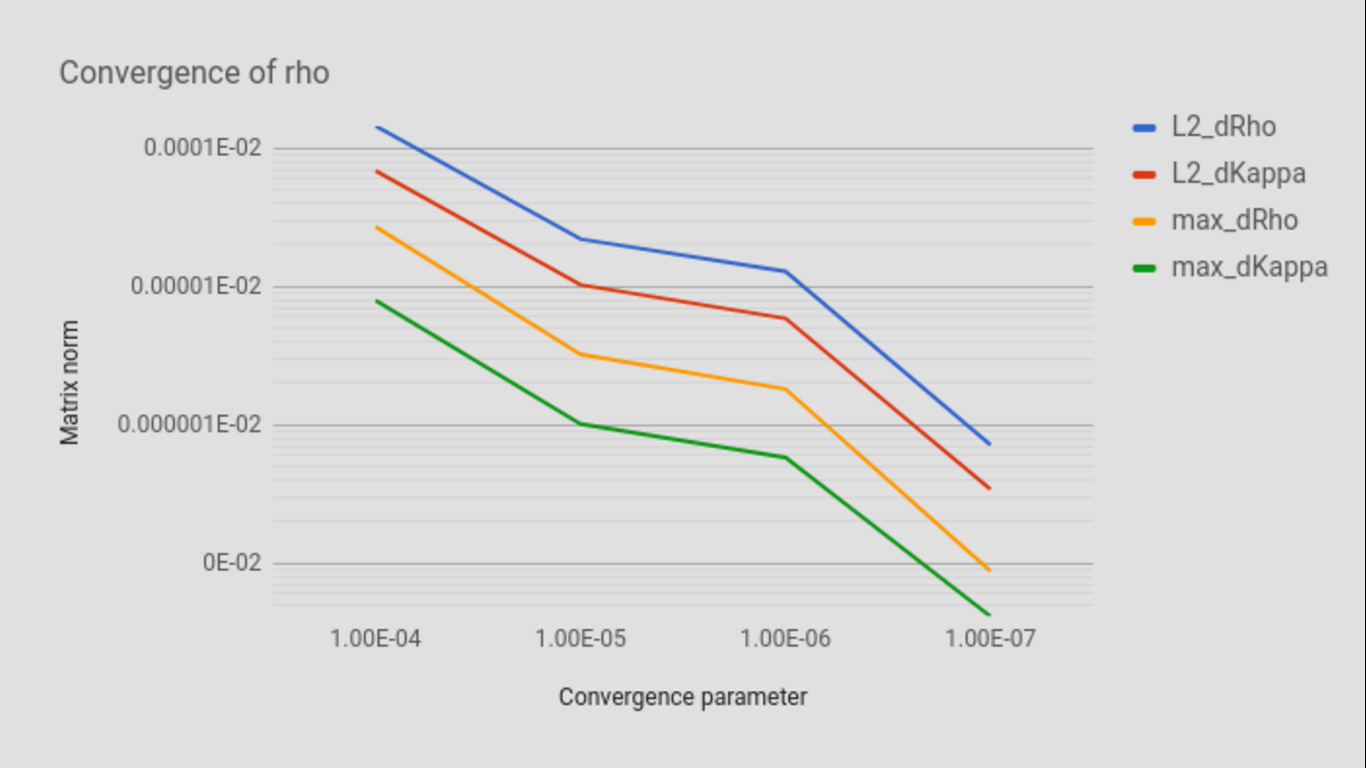
\includegraphics[width=0.7\linewidth]{TeX_files/rho_conv}
\caption{Shown are several different matrix norms for the matrix which is found by subtracting the density matrix of the last iteration from that of the second-to-last iteration. Specifically, these show results for the proton density $\rho$ and the proton pairing density $\kappa$ near the slightly-deformed ground state of $^{240}$Pu.}
\label{fig:rho_conv}
\end{figure}


So what does this mean for us? Specifically, what does this mean for our differentiation by finite differences with various sizes $\delta q$, and how does this change when we start dividing by our $f$s?

We might consider introducing a cutoff on the difference $f_b-f_a$. If we make our cutoff too tight, we start cutting off physics (the tail of the Fermi distribution). If we leave our cutoff too small, we start dividing by numbers that are smaller than the noise in the density matrix.

We know there is an ideal range of values $\delta q$ to use when computing our derivative using finite differences. Too large, and the derivative is unreliable; too small, and the we start crossing into more numerical regions. Suppose we take a value $\delta q = 10^{-3}$ and set our HFODD convergence parameter to $10^{-7}$. Roughly-speaking, then, we would expect that we can set a cutoff for $f_b-f_a$ of something around $10^{-4}$ or so and still obtain reasonable results.

I did this with that $^{240}$Pu calculation for a few different cutoff values. To compare, I computed the exact T=0 inertia. Then I computed the inertia using the same densities which had been computed at T=0, but introducing a fake temperature T=0.05 to calculate the inertia.\footnote{I tried an actual T=0.05 calculation, but it failed to converge and then I forgot about it} The results are in table

\begin{tabular}{|ccc|}
\hline Convergence & $10^{-7}$ &  \\ 
$\delta q$ & $10^{-3}$ &  \\ 
Actual T=0 inertia: & 1.585632E-02 &  \\ \hline
\textbf{Cutoff} & \textbf{Inertia} & \textbf{\% error} \\ \hline
$10^{-4}$ & 1.585205E-02 & -2.692933E-04 \\
$10^{-5}$ & 1.585622E-02 & -6.306634E-06 \\
$10^{-6}$ & 1.585697E-02 & 4.099312E-05 \\
$10^{-7}$ & 1.587771E-02 & 1.348989E-03 \\
$10^{-8}$ & 1.612200E-02 & 1.675546E-02 \\ \hline
\end{tabular} 

\noindent ...So I was a little off on my guess, but I think it illustrates my point.

\section{Fission at finite temperature}

There are several complications associated with considering a nucleus at finite temperature. I'd like to discuss first of all what that even means and why it is significant, and then I'll talk about some of the challenges of this approach.

The idea of considering fission as a finite temperature process stems from trying to develop a picture of induced fission. In induced fission, a neutron which carries some amount of energy is captured by a heavy nucleus in its ground state. That extra energy's gotta go somewhere, but where? In a large nucleus, you have all sorts of places, including any number of single particle excitations, or combination of single particle excitations, or perhaps the entire nucleus moves together as one large collective excitation. Apparently some people went through and did the combinatorics of these possible excitations and decided that the number of them was huge (like, $\sim10^{12}$ huge) \cite{Hilaire2012}. So handling them explicitly just isn't going to work.

Additionally, DFT might not be the best tool for performing finite-temperature calculations. This is because DFT is typically implemented as a variational method, which means it's good for ground state calculations. But highly-deformed nuclei are inherently \textit{not} in their ground state. In fact, this is true even for ``zero-temperature" DFT as well. In practice the results we get are pretty good (most likely the system has time to equilibrate to its ``deformed ground state" at each deformation step, or in other words the path to scission proceeds $\sim$adiabatically), but it's something to definitely keep in mind that (I suspect) could strongly affect your half-life predictions and fragment energies in particular. Furthermore, it's not clear to me how you might correct that should the need arise.

A third thing that Nicolas claims is that the temperature should depend on the actual deformation. I'm not sure where exactly this comes from but it sounds plausible to me.
